%
% 1. process this file with pdflatex
% 2. remind to process it twice otherwise cross-references will be wrong
%
\documentclass[a4paper,12pt]{article}
%
% This is to create hyperlinks for index, URLs and citations (now we can use the
% command \url{...} to create URL with hyperlink)
%
\usepackage{color}
\usepackage[a4paper,colorlinks=true,urlcolor=blue,citecolor=blue,linkcolor=blue,bookmarks=false]{hyperref}
%
% This allows inclusion of pictures. Create figures with PowerPoint and then
% export them individually in PDF, PNG, JPEG, or GIF format (in order of
% preference)
%
\usepackage[pdftex]{graphicx}
\DeclareGraphicsExtensions{.pdf,.png,.jpg,.gif}
%
% phantom space (for abbreviations)
%
\usepackage{xspace}
%
% Definition of margins
%
\usepackage[top=2cm,bottom=2cm,left=2cm,right=2cm]{geometry}
%
% This is needed if you write the report in Italian
%
\usepackage[latin1]{inputenc}% IMPORTANTE! usare codifica ISO-8859-1 per le lettere accentate
%
% Paragraph skip and indent
%
\setlength\parskip{\medskipamount}
\setlength\parindent{0pt}
%
% Frequently used abbreviations.
% - example1: \ie this is an example
% - example2: the \ipsec protocol
%
\def\eg{e.g.\xspace}
\def\ie{i.e.\xspace}
\def\ipsec{IPsec\xspace}
\def\myfig#1{Fig.~#1\xspace}
\def\mytab#1{Tab.~#1\xspace}
\def\rfc#1{RFC-#1\xspace}% usage: \rfc{1422}
%
\begin{document}

\title{Security of Docker containers \\
{\normalsize Report for the Computer Security exam at the Politecnico di Torino}
} \author{Carmine D'Amico (239540) \\
{\normalsize tutor: Antonio Lioy} }
\date{July 2018}
\maketitle

\vfill

\rule{\textwidth}{1pt}

\tableofcontents

\rule{\textwidth}{1pt}

\vfill

\newpage

\section{Introduction}

\newpage

\section{State of the art}

In computer science, the term \textit{virtualisation} is referred to the
creation of virtual computational resources. These resources, normally supplied
as hardware, are instead provided to the user by the operating system through
the creation of a new abstraction layer. OSs, storage devices or network
resources could all be virtualised. Virtualisation can be obtained at different
levels and using different techniques. \par\textit{Virtual machines} have
represented for many years the state of the art of virtualisation, being used in
both consumer and enterprise contexts. In the last years a new technology, based
on \textit{containers}, has started to gain more attention, thanks to its
benefits. Docker is an open source container technology, stepped into the
limelight thanks to its simple interface, which allows to create and control
containers. 

\subsection{From virtual machines...}

With the term virtual machines it is often intended an \textbf{hypervisor-based
virtualisation}, that is a type of virtualisation that acts at hardware level.
Virtual machines (VMs) are established on top of the host operating system,
providing applications with their dependencies, but also an entire guest OS and
a separate kernel. One or more virtual machines can be run on the same machine.
Hypervisors are distinguished in two different types, the one that works
directly on top of the host's hardware (\textbf{bare metal hypervisor}) and the
one that is on top of the host's OS (\textbf{hosted hypervisor}). \par Bare
metal hypervisor provides better performances, not having the overhead of the
extra layer of the host's operating system. It manages directly hardware and the
guest's operating system. On the contrary hosted hypervisor can be manged in an
easier way, running as a normal computer program on the user's operating system.
\par As said before, the hypervisor needs to run on the user's computer, which
is defined as \textit{host machine}, while each virtual machines is called
\textit{guest machine}. It is important to remember this terminology, because it
will be used also in the following, referring to containers. 

% figure of the two types of hypervisor based virtualisation

\subsection{...to containers}

\textbf{Container-based virtualisation} represents another approach to
virtualisation, mainly spread in the last years. Compared to hypervisor-based
virtualisation it results more lightweight, using the host's kernel to run
multiple virtual environments. It virtualises at operating system level (it is
also known as \textbf{OS-level virtualisation}), allowing other applications to
run without installing their own kernel on the host. Containers look like
separated process that just share host's kernel. \par Resources are provided by
the host's OS, together with the container engine. A container engine is the
technology in charge of create and manage containers. \textbf{Docker} represents
one of the most important and most used container engine. A computer program
running into a container can only see the resources allocated to that particular
container. On the same host there could be more than one container, each one
with its personal set of dedicated resources. Although it could be possible to
run more than one computer program inside the same container, it is always
suggested to run only one program per container, in order to separate areas of
concern. It is better to connect multiple containers using user-defined networks
and shared volumes. \par There are many representatives of this container-based
virtualisation approach, like \textit{Linux-VServer}, \textit{OpenVZ} and
\textit{LinuX Container (LXC)}. This last will be better described in the next
section, allowing to better understand the behaviour of containers. 

\begin{figure}[h]
  \centerline{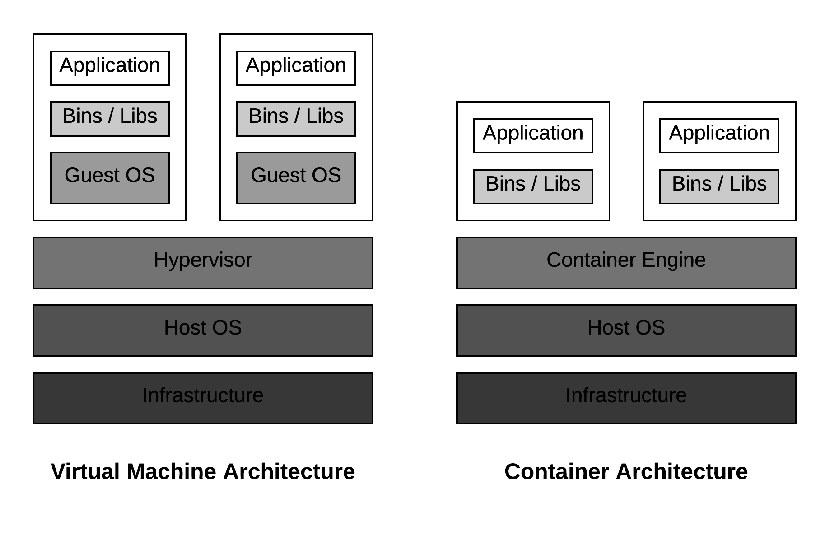
\includegraphics[width=0.7\textwidth]{Architecture-differences-between-virtual-machine-and-container.png}}
  \caption{Architecture differences between virtual machine and container}
  \label{fig:hypervisor_container_difference}
  \end{figure}

% figure of the OS virtualisation

\subsection{LXC}

\textbf{LinuX Containers}, better known as LXC, are an OS-level virtualisation
technique created around 2008. They allow to run multiple isolated Linux
instances (the \textit{containers}), on top of a single host \textit{LXC host},
which shares its Linux kernel. Each container \textit{sees} its own CPU, memory,
network interface, I/O, ecc... \par The isolation among containers is obtained
thanks to some Linux kernel's tools: namespace and cgroups. In the following
subsections these two components will be analysed, both for their importance for
containerisation in general and for the fact that they are also the basic
components in Docker.

\subsubsection{Kernel namespace}

\textbf{Namespaces} allow to create isolated environments, in which each process
that belongs to that particular environment can see global host's resources as
personal isolated resources. In other words they allow to create pool of
processes that think to be the only ones of the system. In this way groups of
processes, that are part of different namespaces, can see different set of
resources. Namespaces work by assigning to different resources the same name in
different namespaces. In the Linux kernel six different type of environments are
implemented:
  \begin{itemize}
    \item PID Namespace
    \item IPC Namespace
    \item UTS Namespace
    \item Network Namespace
    \item User Namespace
    \item Mount Namespace
  \end{itemize} 

\subsubsection{Cgroups}

\textbf{Cgroups} are a kernel tool used to manage processes' resources. They
gather, track and limit processes' usage of resources. It is possible to create
and manage \textit{cgroups} using high level code, assigning PID to a specific
\textit{cgroup}. They represent the fundamental tool to obtain resource
isolation, playing an important role also for the CPU and I/O's scheduling. The
resources that can be limited by Cgroups
are\cite{red_hat_introduction_to_cgroups}:
\begin{itemize}
  \item \textbf{memory} - this subsystem sets limits on memory use by tasks in a
  cgroup and generates automatic reports on memory resources used by those
  tasks. 
  \item \textbf{CPU} - this subsystem uses the scheduler to provide cgroup tasks
  access to the CPU. 
  \item \textbf{CPUacct} - this subsystem generates automatic reports on CPU
  resources used by tasks in a cgroup. 
  \item \textbf{CPUset} - this subsystem assigns individual CPUs (on a multicore
  system) and memory nodes to tasks in a cgroup.
  \item \textbf{blkio} - this subsystem sets limits on input/output access to
  and from block devices such as physical drives (disk, solid state, or USB). 
  \item \textbf{net\_cls} - this subsystem tags network packets with a class
  identifier (classid) that allows the Linux traffic controller (tc) to identify
  packets originating from a particular cgroup task. 
  \item \textbf{net\_prio} - this subsystem provides a way to dynamically set
  the priority of network traffic per network interface. 
  \item \textbf{ns} - the namespace subsystem. 
  \item \textbf{devices} - this subsystem allows or denies access to devices by
  tasks in a cgroup. 
  \item \textbf{freezer} - this subsystem suspends or resumes tasks in a cgroup.
  \item \textbf{perf\_event} - this subsystem identifies cgroup membership of
  tasks and can be used for performance analysis. 
\end{itemize}   

\subsection{Docker}

As today, \textit{Docker} represents the most used computer program for
operating-system-level virtualisation (containerisation). It is developed by
\textbf{Docker, Inc}\cite{docker_official_site} and it was introduced during the
2013's PyCon. During its presentation, \par\textit{Docker} was announced as the
future of Linux Containers\cite{docker_pycon_presentation}, indeed in its first
releases it reiterated many concepts from them, such as \textit{Namespaces} and
\textit{Cgroups}, but providing a simpler user experience and a complete
ecosystem to create and manage containers.\par Docker's success is mainly
addressable to its portability and lightweight nature, that allow to create high
density environments. It is the ideal software in scenarios where continuous
integration and continuous delivery (CI/CD) are required, allowing developers to
not only build their code, but also test their code in any environment type and
as often as possible to catch bugs early in the applications development
life cycle \cite{docker_ci_cd}. 

\subsubsection{History}

\textbf{Docker} was born as an inside project within \textit{dotCloud}, a
platform-as-a-service, later renamed to \textbf{Docker}. Solomon
Hyckes\cite{solomon_hyckes_wiki} was the leader of the project, that was at
first developed with other \textit{dotCloud}'s engineers, like Andrea Luzzardi
and Francois-Xavier Bourlet. The project went public, as said before, during
2013's PyCon and it was released as open source software during the same year.
Always during 2013, \textit{Docker} distanced itself from LXC (exactly with
version 0.9), replacing it with a new execution environment,
\textbf{libcontainer}.\par \textit{Docker} represented a turning point in the
IT industry, as it can be proved by looking ad its adoption. The following is a
list of the milestones achieved by the program from
Wikipedia\cite{docker_history_wiki}:
\begin{itemize}
  \item On September 19, 2013, Red Hat and Docker announced a collaboration
  around Fedora, Red Hat Enterprise Linux, and OpenShift.
  \item In November 2014 Docker container services were announced for the Amazon
  Elastic Compute Cloud (EC2).
  \item On November 10, 2014, Docker announced a partnership with
  Stratoscale.
  \item On December 4, 2014, IBM announced a strategic partnership with Docker
  that enables Docker to integrate more closely with the IBM Cloud.
  \item On June 22, 2015, Docker and several other companies announced that they
  are working on a new vendor and operating-system-independent standard for
  software containers.
  \item As of October 24, 2015, the project had over 25,600 GitHub stars (making
  it the 20th most-starred GitHub project), over 6,800 forks, and nearly 1,100
  contributors.
  \item A May 2016 analysis showed the following organisations as main
  contributors to Docker: The Docker team, Cisco, Google, Huawei, IBM,
  Microsoft, and Red Hat.
  \item On October 4, 2016, Solomon Hykes announced InfraKit as a new
  self-healing container infrastructure effort for Docker container
  environments.
  \item A January 2017 analysis of LinkedIn profile mentions showed Docker
  presence grew by 160\% in 2016.[30] The software has been downloaded more than
  13 billion times as of 2017.

\end{itemize}   

\subsubsection{Docker's architecture\cite{docker_architecture}}

\textbf{Docker} follows a client-server architecture, where three main
components can be distinguished (\myfig{\ref{fig:docker-architecture}}):
\begin{itemize}
  \item The server, which is a daemon process (called \textbf{dockerd}) running
  on the host's machine. It is in charge of create and manage Docker's objects.
  \item A set of interfaces conformed to REST architectural style, that enable
  programs to communicate with the server, sending instructions.
  \item A command line interface (CLI) client, that allows the user to interact
  with Docker using the REST API through their terminal.
\end{itemize}   

\begin{figure}[h]
  \centerline{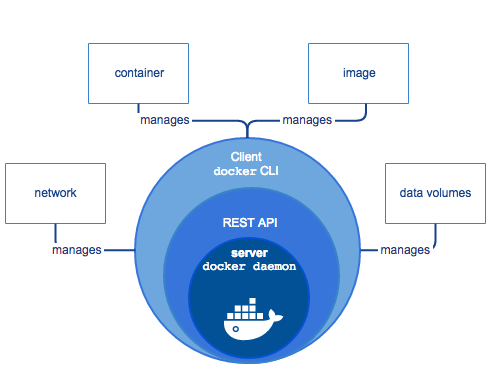
\includegraphics[width=0.7\textwidth]{engine-components-flow.png}}
  \caption{Docker's architecture.}
  \label{fig:docker-architecture}
  \end{figure}

\subsubsection{Docker's objects\cite{docker_objects}}

Docker's workflow includes the interaction with many special purpose objects,
created and managed by \textbf{containerd}:
\begin{itemize}
  \item \textbf{IMAGES} are the basic components involved in the creation of a
  Docker's container, containing all the instructions that the daemon has to
  follow. An image can be created from scratch or it can be based on already
  existing images (for example on the image of \textit{nginx}), where other
  needed components are installed. A \textit{Dockerfile} is a special file, that
  follows a very simple syntax, which includes all the steps that must be
  followed in order to create an image. Each instruction represents a layer in
  the image. When a new layer is inserted (modifying the \textit{Dockerfile})
  and a container is rebuilt, only the new layer is rebuilt, speeding up the
  deployment's process.\par Docker images are stored inside registries, that can
  be private or public. The two most famous public registries are \textit{Docker
  Cloud} and \textit{Docker Hub}, the latter is the default one visited by
  Docker for searching images.   
  \item \textbf{CONTAINERS} represent the the runnable instances of images.
  The relationship between images and containers could be compared to the
  relationship between classes and objects in an object-oriented programming
  language. A container can be connected to the network or to a storage and it
  can be defined by its image or by the configurations indicated starting
  it.\par When a container is started Docker searches locally for all the needed
  images (downloading them from online public registries if necessary), then a
  read/write file system is allocated, where the container can create or modifies
  file or directories. By default a container can be connected to the external
  network using the host's connection. When a container is stopped  any changes
  to its state that are not stored in persistent storage disappear.
  \item \textbf{SERVICES} are supported from version 1.12 of Docker. They allow
  to run containers across different daemons. A series of daemons connected
  between them compose a \textit{swarm} and they all communicate between them
  using Docker's REST API. A user can defines \textit{swarm}'s configurations,
  like the number of \textit{service}'s replica available. A \textit{service} is
  seen from the external as a single application.
\end{itemize}   

\subsubsection{Security by default}

As stated before, Docker uses some LXC's features, like namespaces and control
groups. These components provide a series of security features to Docker, like
isolation and resource accounting. \par With namespaces each process running
inside a container can't see or interact with processes belonging to other
containers or to the host system, creating a first form of isolation. Moreover,
by default containers can't even interact between each other using their network
interfaces, because each one has its own network stack. It is possible, anyway,
to setup the host to make network interaction admissible, specifying containers'
public ports or creating \textit{links}\cite{legacy_container_links} to enable
IP traffic between them.\par Control groups are essential in order to prevent
denial-of-service attacks (DoS attacks). Implementing resource accounting and
limiting, indeed,  they don't allow a single container to bring down the host
system exhausting one or more sources (CPU, memory, disk I/O, ecc...). This is
particularly important in a multi-tenant system, where more than one container
works together. 


\newpage

\section{Hardening Docker}

\newpage

\begin{thebibliography}{99}

 
\bibitem{red_hat_introduction_to_cgroups}
\url{https://access.redhat.com/documentation/en-us/red_hat_enterprise_linux/6/html/resource_management_guide/ch01}

\bibitem{docker_official_site}
\url{https://www.docker.com/}

\bibitem{docker_pycon_presentation}
\url{https://www.youtube.com/watch?v=wW9CAH9nSLs}

\bibitem{solomon_hyckes_wiki}
\url{https://en.wikipedia.org/wiki/Solomon_Hykes}

\bibitem{docker_ci_cd}
\url{https://www.docker.com/use-cases/cicd}

\bibitem{docker_history_wiki}
\url{https://en.wikipedia.org/wiki/Docker_(software)#History}

\bibitem{docker_architecture}
\url{https://docs.docker.com/engine/docker-overview/#docker-architecture}

\bibitem{docker_objects}
\url{https://docs.docker.com/engine/docker-overview/#docker-objects}

\bibitem{legacy_container_links}
\url{https://docs.docker.com/network/links/}

\end{thebibliography}

\end{document}
%
% Before delivering your report, don't forget to run a spell checker, such as
% aspell (with a UK-english dictionary)
%
